\documentclass[11pt,a4paper]{article}
\usepackage[margin=23mm,headheight=16pt]{geometry}
\usepackage[T1]{fontenc}
\usepackage{tgpagella}
\usepackage{amsmath,amssymb,amsthm,mathtools,bm,microtype,booktabs,tabularx,longtable,enumitem}
\usepackage{tikz}
\usetikzlibrary{arrows.meta,positioning,calc,patterns,decorations.pathmorphing}
\usepackage{xcolor,fancyhdr,hyperref}
\definecolor{deepblue}{RGB}{25,50,99}\definecolor{purple}{RGB}{104,69,170}\definecolor{softblue}{RGB}{227,238,249}
\hypersetup{colorlinks=true,linkcolor=deepblue,urlcolor=deepblue}
\pagestyle{fancy}\fancyhf{}\fancyhead[L]{\small Measurement Backaction and Quantum Trajectories}\fancyhead[R]{\small Quantum Companion VII}\fancyfoot[C]{\thepage}
\setlength{\parskip}{5pt}\setlength{\parindent}{0pt}
\setcounter{secnumdepth}{3}
\newtheorem{example}{Worked Example}\newtheorem{remark}{Physical qualification}
\newcommand{\tr}{\operatorname{Tr}}\newcommand{\D}{\mathcal D}\newcommand{\kb}{k_{\mathrm B}}\newcommand{\E}{\mathbb E}\newcommand{\Ha}{\mathcal H}\newcommand{\ket}[1]{|#1\rangle}\newcommand{\bra}[1]{\langle#1|}
\begin{document}
\begin{center}
{\Large\bfseries\color{deepblue} Open Quantum Systems, Measurement Backaction\\ and Quantum Trajectories}\par\medskip
{\large Chapter VII: Rubidium Fluorescence, Lindblad Dynamics,\\ Particle Loss and Continuous Many-Body Monitoring}\par\smallskip
{\small Advanced Quantum Physics Companion --- append-only series; Chapters I--VI preserved unchanged}\par
\end{center}
\begin{abstract}
Starting from rubidium-87 internal states and site-resolved many-boson models, this chapter derives the Gorini--Kossakowski--Sudarshan--Lindblad equation, measurement instruments, quantum-jump trajectories and diffusive stochastic master equations. Explicit calculations examine spontaneous emission, local number monitoring, one- and two-body losses, fluorescence-induced dephasing, photon recoil, the quantum Zeno regime and measurement-driven changes to coherence and entanglement. Each calculation distinguishes a detector-conditioned trajectory from the unconditional density matrix. We provide numerical scales, validation tests, original diagrams, additional exercises and scientific references. All examples are controlled effective models rather than claims that a specific Tiangong experiment implemented site-resolved continuous readout.
\end{abstract}
\tableofcontents\clearpage
\section{From coherent matter waves to open quantum dynamics}
The preceding chapters distinguish the electron's $5s$ orbital from the motional states of entire $^{87}$Rb atoms. An optical lattice supports a many-body Bose--Hubbard Hamiltonian
\begin{equation}
H_{\rm BH}=-J\sum_{\langle i,j\rangle}(a_i^\dagger a_j+a_j^\dagger a_i)+\frac U2\sum_i n_i(n_i-1)+\sum_i V_i n_i.
\end{equation}
The evolution of an isolated system is unitary: $\dot\rho=-i[H,\rho]/\hbar$. A fluorescence-imaged lattice instead interacts with light and other environmental degrees of freedom. If these degrees of freedom are discarded, the reduced dynamics may be irreversible. A time-homogeneous, trace-preserving completely positive Markovian generator has the standard GKSL form:
\begin{equation}\label{eq:gksl}
\boxed{\dot\rho=-\frac{i}{\hbar}[H,\rho]+\sum_\mu\left(L_\mu\rho L_\mu^\dagger-\frac12\{L_\mu^\dagger L_\mu,\rho\}\right).}
\end{equation}
We abbreviate the dissipator as $\D[L]\rho=L\rho L^\dagger-\tfrac12\{L^\dagger L,\rho\}$. The operators $L_\mu$ contain square roots of rates. A phenomenological Lindbladian requires validity checks: time-local Markov approximation, appropriate coarse graining, resolved or unresolved scattering channels, and correct treatment of losses.
\begin{figure}[ht]\centering
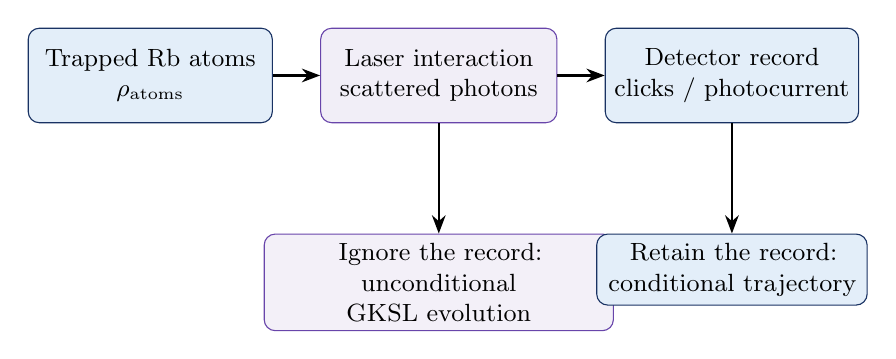
\begin{tikzpicture}[>=Stealth,node distance=6mm, every node/.style={font=\small}]
\node[draw=deepblue,fill=softblue,rounded corners,minimum width=3.1cm,minimum height=12mm,align=center] (s) {Trapped Rb atoms\\$\rho_{\rm atoms}$};
\node[draw=purple,fill=purple!9,rounded corners,minimum width=3.0cm,minimum height=12mm,align=center,right=of s] (p) {Laser interaction\\scattered photons};
\node[draw=deepblue,fill=softblue,rounded corners,minimum width=3.0cm,minimum height=12mm,align=center,right=of p] (d) {Detector record\\clicks / photocurrent};
\draw[->,thick] (s)--(p);\draw[->,thick] (p)--(d);
\node[below=14mm of p,draw=purple,fill=purple!8,rounded corners,align=center,text width=4.2cm] (u) {Ignore the record:\\unconditional GKSL evolution};
\node[below=14mm of d,draw=deepblue,fill=softblue,rounded corners,align=center,text width=3.2cm] (c) {Retain the record:\\conditional trajectory};
\draw[->,thick] (p)--(u);\draw[->,thick] (d)--(c);
\end{tikzpicture}
\caption{Measurement is a physical coupling. A recorded outcome conditions the atomic state; an unread environment produces an averaged density matrix.}
\end{figure}
\section{Derivation with Kraus operators}
Suppose there is one monitored jump channel $L$ and a small time interval $dt$. Define
\begin{equation}
M_1=\sqrt{dt}\,L,\qquad M_0=I-\frac{iH}{\hbar}dt-\frac12 L^\dagger L\,dt.
\end{equation}
Then $M_0^\dagger M_0+M_1^\dagger M_1=I+O(dt^2)$. If the outcome is unknown, the map is $\rho\mapsto M_0\rho M_0^\dagger+M_1\rho M_1^\dagger$. Expanding through first order yields $\dot\rho=-i[H,\rho]/\hbar+\D[L]\rho$. Multiple channels are added analogously. This construction establishes trace preservation; complete positivity follows from the Kraus map at each increment.
\begin{example}[Trace preservation]
By cyclicity, $\tr(L\rho L^\dagger)=\tr(L^\dagger L\rho)$ and $\tr\{L^\dagger L,\rho\}=2\tr(L^\dagger L\rho)$. Therefore $\tr\D[L]\rho=0$ and $\frac{d}{dt}\tr\rho=0$. The commutator also has zero trace.
\end{example}
\begin{remark}
The jump-operator representation is not unique, and different environmental measurement schemes (unravelings) can realize the same unconditional generator. An equation for $\rho$ does not by itself specify an actual experimental detection record.
\end{remark}
\section{Internal Rb-87 fluorescence as a quantum-jump channel}
In an ideal two-level approximation with excited state $\ket e$ and ground state $\ket g$, define $\sigma_-=\ket g\bra e$ and $L=\sqrt\Gamma\,\sigma_-$. Without driving, $\dot\rho=\Gamma\D[\sigma_-]\rho$. In the ordered basis $(e,g)$,
\begin{align}
\dot\rho_{ee}&=-\Gamma\rho_{ee}, & \dot\rho_{gg}&=\Gamma\rho_{ee},\\
\dot\rho_{eg}&=-\frac\Gamma2\rho_{eg}.&&
\end{align}
Thus $\rho_{ee}(t)=\rho_{ee}(0)e^{-\Gamma t}$ and $\rho_{eg}(t)=\rho_{eg}(0)e^{-\Gamma t/2}$.
\begin{example}[Rubidium D2 decay]
For the D2 line near $780.241\,$nm, the excited-state lifetime is approximately $\tau=26.24\,$ns, so $\Gamma=1/\tau\simeq3.81\times10^7\,$s$^{-1}$ and $\Gamma/(2\pi)\simeq6.06\,$MHz. After $t=\tau$, an initially excited ideal two-level atom has excited-state probability $e^{-1}=0.3679$. Real Rb-87 fluorescence cycling involves hyperfine manifolds, polarization selection rules, repumping and sometimes dark states: a perfect two-level reduction must be justified.
\end{example}
\begin{example}[Conditional click and no-click paths]
For a detected photon during $dt$, the state is $\rho_\mathrm{click}=L\rho L^\dagger/\tr(L^\dagger L\rho)$, with probability $p_\mathrm{click}=dt\,\tr(L^\dagger L\rho)$. If no click is recorded, the state is $M_0\rho M_0^\dagger/\tr(M_0\rho M_0^\dagger)$. The non-Hermitian effective Hamiltonian is $H_\mathrm{eff}=H-i\hbar L^\dagger L/2$. No-click conditioning changes the weights of excited and ground components even though no photon was seen.
\end{example}
\section{Quantum trajectories and stochastic jump simulation}
For a pure normalized conditioned state $\ket\psi$, one timestep of the Monte Carlo wavefunction method uses $p_\mu=dt\bra\psi L_\mu^\dagger L_\mu\ket\psi$. With probability $p_\mu$, a jump occurs: $\ket\psi\mapsto L_\mu\ket\psi/\|L_\mu\ket\psi\|$. Otherwise the state evolves under $H_\mathrm{eff}=H-i\hbar\sum_\mu L_\mu^\dagger L_\mu/2$ and is renormalized. Averaging independent conditional states reconstructs $\rho(t)$ when detection channels are modeled consistently.
\begin{example}[Survival without a photon]
For a two-level system initially in $\ket e$ and no re-excitation, the waiting-time distribution to the first emitted photon is $f(t)=\Gamma e^{-\Gamma t}$, its survival function is $S(t)=e^{-\Gamma t}$ and its mean waiting time is $1/\Gamma$. This is a single-decay model, not the continuously driven resonant-fluorescence process with repeated jumps.
\end{example}
\section{Fluorescence-induced dephasing in a lattice}
For a spatially resolved, idealized nondestructive number measurement, use $L_i=\sqrt\gamma\,n_i$. Consider a single atom shared between left and right sites, $\ket\psi=(\ket L+\ket R)/\sqrt2$. The two site-monitoring channels cause the off-diagonal element to obey
\begin{equation}\label{eq:dephasing}
\frac{d}{dt}\rho_{LR}=-\gamma\rho_{LR}\quad\Longrightarrow\quad\rho_{LR}(t)=\frac12e^{-\gamma t}.
\end{equation}
Populations are unchanged by this pure-dephasing model. The probability distribution for which site holds the atom remains $(1/2,1/2)$, but its phase coherence disappears in the unread ensemble.
\begin{example}[Visibility suppression]
Let $\gamma=50\,$s$^{-1}$ and $t=20\,$ms. The normalized off-diagonal coherence is reduced by $e^{-\gamma t}=e^{-1}\simeq0.3679$. For a balanced two-mode ideal interference pattern, fringe visibility falls by the same factor, provided that no other process affects the populations or detection contrast.
\end{example}
\begin{remark}
The Lindblad operator $n_i$ is an effective ideal local monitoring model. Real fluorescence includes nonlocal optical resolution, recoil heating, internal transitions and possibly atom loss. For an unresolved detector one may need a collective operator $\sum_i f_i n_i$; two sites that scatter indistinguishably need not fully decohere relative to one another.
\end{remark}
\section{Decoherence versus number localization}
\begin{figure}[ht]\centering
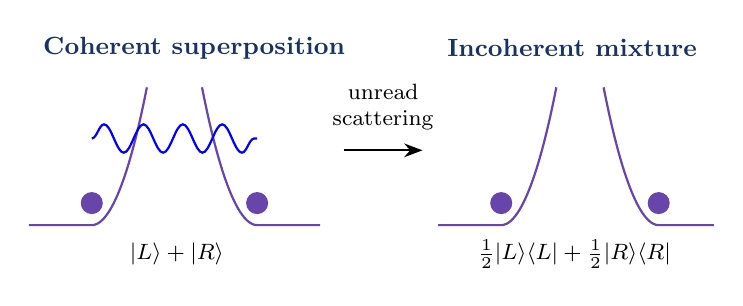
\begin{tikzpicture}[>=Stealth,scale=1]
\node[font=\small\bfseries,deepblue] at (2.4,2.6) {Coherent superposition};
\draw[purple,thick] (.3,.35) parabola bend (1.1,.35) (1.8,2.1);\draw[purple,thick] (2.5,2.1) parabola bend (3.2,.35) (4,.35);
\fill[purple] (1.1,.63) circle (.14);\fill[purple] (3.2,.63) circle (.14);
\draw[blue,thick,decorate,decoration={snake,amplitude=1.8mm,segment length=5mm}] (1.1,1.45)--(3.2,1.45);
\node[font=\footnotesize] at (2.18,-.02) {$|L\rangle+|R\rangle$};
\draw[->,thick] (4.3,1.3)--(5.3,1.3);\node[align=center,font=\footnotesize] at (4.8,1.85) {unread\\scattering};
\node[font=\small\bfseries,deepblue] at (7.2,2.6) {Incoherent mixture};
\draw[purple,thick] (5.5,.35) parabola bend (6.3,.35) (7,2.1);\draw[purple,thick] (7.6,2.1) parabola bend (8.3,.35) (9,.35);
\fill[purple] (6.3,.63) circle (.14);\fill[purple] (8.3,.63) circle (.14);
\node[font=\footnotesize] at (7.23,-.02) {$\tfrac12|L\rangle\langle L|+\tfrac12|R\rangle\langle R|$};
\end{tikzpicture}
\caption{Unobserved which-site information can destroy relative coherence without changing the diagonal position probabilities. Schematic, not a literal image of atomic orbitals.}
\end{figure}
In a number-eigenstate basis $\ket{\mathbf n}$, the dissipator from local $L_i=\sqrt\gamma n_i$ gives
\begin{equation}\label{eq:manydephasing}
\bra{\mathbf n}\mathcal L_\mathrm{deph}(\rho)\ket{\mathbf m}
=-\frac\gamma2\sum_i(n_i-m_i)^2\rho_{\mathbf n\mathbf m}.
\end{equation}
Diagonal populations are unchanged, while coherences between number patterns decay according to their distinguishability. The formula follows from $n_i\ket{\mathbf n}=n_i\ket{\mathbf n}$.
\begin{example}[Two-boson coherences]
For the states $\ket{2,0}$ and $\ket{1,1}$, squared occupation differences sum to $1^2+(-1)^2=2$, so their off-diagonal element decays at rate $\gamma$. For $\ket{2,0}$ and $\ket{0,2}$ the sum is $2^2+(-2)^2=8$, giving decay rate $4\gamma$. The environment distinguishes the latter pair much more strongly.
\end{example}
\section{One-body and two-body atomic loss}
A genuine loss channel removes atoms from the retained system, and the appropriate model may require multiple particle-number sectors. For local one-body loss, take $L_i^{(1)}=\sqrt{\kappa_1}a_i$. For pair loss, take $L_i^{(2)}=\sqrt{\kappa_2}a_i^2$. The convention chosen means the pair-event rate in number state $\ket n$ is $\kappa_2n(n-1)$.
\begin{align}
\frac d{dt}\langle N\rangle\bigg|_{1\mathrm{b}}&=-\kappa_1\langle N\rangle,\\
\frac d{dt}\langle N\rangle\bigg|_{2\mathrm{b}}&=-2\kappa_2\sum_i\langle n_i(n_i-1)\rangle.
\end{align}
The second expression depends on onsite pair correlations and cannot in general be closed using only $\langle n_i\rangle$.
\begin{example}[One-body lifetime]
If $N(0)=20{,}000$ atoms and each is lost independently at rate $\kappa_1=0.01\,$s$^{-1}$, the mean population is $\langle N(t)\rangle=20{,}000e^{-0.01t}$. At $t=10\,$s, the mean is approximately $18{,}097$. This is a hypothetical illustrative rate, not a Tiangong measurement.
\end{example}
\begin{example}[Pair-loss rate of a Fock state]
One well with three atoms has $\bra3 a^{\dagger2}a^2\ket3=3(3-1)=6$. Its pair-event rate is $6\kappa_2$, and the initial mean atom loss rate is $12\kappa_2$. The jump maps $\ket3$ to a normalized $\ket1$ state, not $\ket2$.
\end{example}
\section{Continuous diffusive measurement and stochastic master equations}
Photon counting gives jumps; homodyne-like monitoring gives a continuous noisy signal. For an idealized Hermitian observable $A=A^\dagger$, define $L=\sqrt\gamma A$ and efficiency $0\le\eta\le1$. A conventional It\^o stochastic master equation is
\begin{equation}\label{eq:sme}
\boxed{d\rho_c=-\frac i\hbar[H,\rho_c]dt+\gamma\D[A]\rho_c\,dt+\sqrt{\eta\gamma}\,\mathcal H[A]\rho_c\,dW,}
\end{equation}
where $dW$ is a Wiener increment with $\E[dW]=0$, $dW^2=dt$, and
\begin{equation}
\mathcal H[A]\rho=A\rho+\rho A-2\tr(A\rho)\rho.
\end{equation}
An associated normalized measurement record is
\begin{equation}\label{eq:record}
dY=2\sqrt{\eta\gamma}\,\tr(A\rho_c)dt+dW.
\end{equation}
Averaging over the innovation noise gives the unconditional GKSL equation. The stochastic state $\rho_c$ changes differently for different detection records.
\begin{example}[Efficiency matters]
At $\eta=0$ there is no available record and the conditional innovation term vanishes, but dephasing $\gamma\D[A]\rho$ remains. At $\eta=1$ all information in this ideal channel is available. A poor collection efficiency does not undo the physical measurement backaction induced by scattered photons.
\end{example}
\section{Quantum Zeno suppression of tunneling}
Take one atom in two sites with Hamiltonian $H=-J\sigma_x$ and local which-site dephasing at off-diagonal rate $\gamma$. Writing $z=\rho_{LL}-\rho_{RR}$ and $y=\operatorname{Im}\rho_{LR}$ yields (with one consistent sign convention)
\begin{equation}
\dot z=\frac{4J}{\hbar}\,y,\qquad \dot y=-\frac J\hbar z-\gamma y.
\end{equation}
Thus $\ddot z+\gamma\dot z+4(J/\hbar)^2 z=0$. In the strongly monitored regime $\gamma\gg J/\hbar$, the slow decay rate of the imbalance is approximately
\begin{equation}\label{eq:zeno}
\Gamma_{\rm Z}\simeq\frac{4J^2}{\hbar^2\gamma}.
\end{equation}
This is a quantum Zeno regime: stronger monitoring slows intersite population transfer. It is not perfect freezing at finite monitoring rate.
\begin{example}[A numerical Zeno estimate]
For $J/h=100\,$Hz, $J/\hbar=2\pi\times100\,$s$^{-1}$. Choose $\gamma=2\pi\times10{,}000\,$s$^{-1}$. Then $\Gamma_{\rm Z}\approx25.1\,$s$^{-1}$. The resulting slow-time constant is approximately $39.8\,$ms. The strong-monitoring assumption $\gamma/(J/\hbar)=100$ is satisfied.
\end{example}
\section{What measurement does to entanglement}
An individual monitored trajectory can become pure and strongly localized, while the unconditional state becomes mixed. An observer's missing measurement record and a physical loss of atoms are not the same phenomenon. For a pure bipartite state, the entropy $S_A=-\tr(\rho_A\ln\rho_A)$ measures spatial-mode entanglement. If the global unconditional state is mixed, $S(\rho_A)$ alone is not a valid entanglement monotone; classical and quantum correlations contribute.
Consider an initial Bell-like one-atom mode state $\ket{\psi_+}=(\ket L+\ket R)/\sqrt2$. With local unread which-site monitoring, the density matrix becomes
\begin{equation}
\rho(t)=\frac12\begin{pmatrix}1&e^{-\gamma t}\\e^{-\gamma t}&1\end{pmatrix}.
\end{equation}
Its one-particle coherence is $\rho_{LR}(t)=e^{-\gamma t}/2$. The normalized global purity is
\begin{equation}\tr\rho(t)^2=\frac12(1+e^{-2\gamma t}).\end{equation}
\begin{example}[Purity at one dephasing time]
At $\gamma t=1$, the purity is $(1+e^{-2})/2\approx0.56767$. This is a direct observable of mixing. For a fixed one-atom two-mode system, local operational accessibility of entanglement requires care with particle-number superselection; do not infer a resource claim from mode entropy alone.
\end{example}
\section{Recoil heating and limits of a dephasing-only model}
An emitted photon carries momentum of magnitude $\hbar k$. The associated atom recoil energy is $E_R=\hbar^2k^2/(2M)=h^2/(2M\lambda^2)$. For $^{87}$Rb at $\lambda\simeq780\,$nm, $E_R/h\approx3.77\,$kHz, and $E_R/k_B\approx181\,$nK. Absorption and emission can each impart recoil. Depending on beam directions and angular emission, heating rates depend on geometry and optical-pumping details.
\begin{example}[Energy scale of 100 recoils]
One hundred independent recoil-energy contributions correspond nominally to $100E_R/k_B\simeq18.1\,\mu$K. This is only a scale comparison: efficient imaging schemes apply cooling that counteracts recoil; summing recoils does not automatically predict a final equilibrium temperature.
\end{example}
\section{Detector models, photostatistics and readout fidelity}
A fluorescence detector typically collects only a fraction of emitted photons. Let $R_{\rm sc}$ be the photon-scattering rate, $\eta_{\rm coll}$ collection efficiency and $\eta_{\rm det}$ downstream detection efficiency. In a crude independent-photon model, the mean detected count in interval $t$ is $\bar n_d=R_{\rm sc}\eta_{\rm coll}\eta_{\rm det}t$, and the zero-count probability for a Poisson signal is $e^{-\bar n_d}$. Background counts, atom loss, optical pumping and imperfect point-spread-function separation modify this. High fluorescence counts therefore do not automatically imply faithful QND readout.
\begin{example}[Photon collection model]
If $R_{\rm sc}=10^5\,$s$^{-1}$, total efficiency $0.05$, and exposure $t=10\,$ms, the expected detected photon number is $50$. Ignoring background, the probability of seeing zero photons is $e^{-50}\approx1.93\times10^{-22}$. But actual number resolution may still fail through parity projection or atom hopping and loss.
\end{example}
\section{Numerical laboratory: minimal validation protocol}
For a finite-dimensional truncated bosonic lattice, construct $H$ and jumps $L_\mu$ and integrate the GKSL equation. Recommended validation gates:
\begin{enumerate}[label=\textbf{V\arabic*.},leftmargin=*]
\item Verify $\tr\rho(t)=1$ to numerical tolerance and $\rho=\rho^\dagger$.
\item Check minimum eigenvalue of $\rho(t)$ does not show significant negative values.
\item Verify $\langle N\rangle$ is constant for pure number monitoring and decreases for physical loss.
\item Compare analytic two-site dephasing $e^{-\gamma t}$ with numerical evolution.
\item Reconstruct unconditional $\rho(t)$ by averaging jump trajectories; report sampling error.
\item Check timestep convergence and finite Fock-space cutoff effects for loss and driving.
\item Distinguish all-site monitoring from a collective measurement channel.
\item Validate conditioned trajectories against recorded click/no-click probabilities.
\end{enumerate}
\section{Appendix A: derivation of many-site dephasing decay}
Let $L_i=\sqrt\gamma n_i$ and $\ket{\mathbf n},\ket{\mathbf m}$ be joint eigenstates of all $n_i$. Then
\begin{align*}
\bra{\mathbf n}\D[L_i]\rho\ket{\mathbf m}
&=\gamma n_i m_i\rho_{\mathbf n\mathbf m}-\frac\gamma2(n_i^2+m_i^2)\rho_{\mathbf n\mathbf m}\\
&=-\frac\gamma2(n_i-m_i)^2\rho_{\mathbf n\mathbf m}.
\end{align*}
Summing over sites yields Eq.~\eqref{eq:manydephasing}. This makes the environmental distinguishability of number configurations explicit.
\section{Appendix B: derivation of loss equations}
For any observable $O$, the dissipative part satisfies $\frac{d}{dt}\langle O\rangle=\sum_\mu\langle L_\mu^\dagger O L_\mu-\frac12\{L_\mu^\dagger L_\mu,O\}\rangle$. Take $O=N=\sum_i n_i$ and $L_i=\sqrt{\kappa_1}a_i$. Since $[N,a_i]=-a_i$, it follows that $\dot{\langle N\rangle}=-\kappa_1\langle N\rangle$. With $a_i^2$, the commutator is $[N,a_i^2]=-2a_i^2$, yielding the two-body loss relation above. This is exact within the specified effective jump model.
\section{Appendix C: a step-by-step conditional photon simulation}
Start with normalized $\ket{\psi_0}$, time step $dt$, and jump set $\{L_\mu\}$. Compute probabilities\par\vspace{-5pt}\[p_\mu=dt\bra\psi L_\mu^\dagger L_\mu\ket\psi.\]\vspace{-8pt}Draw a uniform random number $u$. If it falls into one of the event intervals, apply and normalize the associated $L_\mu$. Otherwise propagate $\ket\psi$ with $I-iH_{\rm eff}dt/\hbar$ and normalize. Store record time, channel label and observables. Repeat over trajectories and compare the ensemble mean with direct GKSL integration. For meaningful estimates of rare events, assess Monte Carlo uncertainty rather than treating one record as typical.
\section{Additional problems}
\begin{enumerate}[label=\textbf{P\arabic*.},leftmargin=*]
\item Derive the Bloch equations for a driven two-level atom with radiative damping and resonant Rabi frequency $\Omega$.
\item Prove the derivative of $\tr\rho^2$ for a two-site number-dephasing model and identify its sign for a pure initial bonding state.
\item Compute the jump probabilities for $\ket{2,1}$ under site-local one-body and two-body losses.
\item Derive Eq.~\eqref{eq:manydephasing} for arbitrary $L$ sites with nonuniform rates $\gamma_i$.
\item Show that collective monitoring with $L=\sqrt\gamma(n_L+n_R)$ does not distinguish $\ket L$ and $\ket R$ in a fixed-$N=1$ subspace.
\item Calculate the two-site imbalance equation and the quantum Zeno slow rate for $\gamma\gg J/\hbar$.
\item Explain why a conditional pure-state trajectory and a mixed unconditional density matrix can describe the same experimental apparatus.
\item Derive the second-order photon-count distribution for a single-decay atom and distinguish it from driven fluorescence.
\item Simulate single-boson hopping with local dephasing and validate positivity for $0\le\gamma t\le10$.
\item Compute the recoil-frequency scale for $^{87}$Rb at wavelengths $780$ and $1064\,$nm.
\item Generalize the ideal homodyne record Eq.~\eqref{eq:record} to a collective number operator $A=n_1+n_2$ and discuss whether it identifies a site.
\item Design an experiment that separately estimates atom loss, induced heating and site occupation readout errors.
\end{enumerate}
\section{References and source notes}
\begin{enumerate}[leftmargin=*]
\item A. J. Daley, ``Quantum trajectories and open many-body quantum systems,'' \emph{Advances in Physics} \textbf{63}, 77--149 (2014), doi:10.1080/00018732.2014.933502.
\item W. S. Bakr et al., ``A quantum gas microscope for detecting single atoms in a Hubbard-regime optical lattice,'' \emph{Nature} \textbf{462}, 74--77 (2009), doi:10.1038/nature08482.
\item D. A. Steck, \emph{Rubidium 87 D Line Data}, version 2.3.4 (2025), \url{https://steck.us/alkalidata/}.
\item A. N. Jordan et al., ``Measuring fluorescence to track a quantum emitter's state: a theory review,'' \emph{Contemporary Physics} (2020), doi:10.1080/00107514.2020.1747201.
\item ``An Introduction to Monitored Quantum Systems and Quantum Trajectories: Spectrum, Typicality, and Phases,'' \emph{Progress of Theoretical and Experimental Physics} \textbf{2026}, 052A01 (2026). The local number-monitoring jump model is presented as an idealized effective description.
\item G. Lindblad, ``On the generators of quantum dynamical semigroups,'' \emph{Communications in Mathematical Physics} \textbf{48}, 119--130 (1976).
\item V. Gorini, A. Kossakowski and E. C. G. Sudarshan, ``Completely positive dynamical semigroups of $N$-level systems,'' \emph{Journal of Mathematical Physics} \textbf{17}, 821--825 (1976).
\end{enumerate}
\end{document}
